\section{内存模型和原子}
如果我们想成为并行程序员,内存一致性并不是一个深奥的概念。 
它帮助我们确保数据在我们需要的时候出现在我们需要的地方,并且它的值是我们所期望的。 
本章揭示了我们需要掌握的关键知识,以确保我们的程序正确运行。 这个主题并不是 SYCL 独有的。

对于任何想要允许并发更新内存的程序员来说,
对编程语言的内存(一致性)模型有基本的了解是必要的(无论这些更新是否来自同一Kernel、多个设备或两者中的多个Work-Items)。 
无论内存如何分配都是如此,无论我们选择使用Buffer还是USM分配,本章的内容对我们来说都同样重要。

在前面的章节中,我们重点关注简单Kernel的开发,其中Work-Items要么对完全独立的数据进行操作,
要么使用可以使用语言和/或库功能直接表达的结构化通信模式共享数据。 
当我们转向编写更复杂和更现实的Kernel时,我们可能会遇到Work-Items可能需要以不太结构化的方式进行通信的情况 - 
了解内存模型如何与 SYCL 语言功能以及我们目标硬件的功能相关。 设计正确、可移植、高效的程序的必要前提。

\begin{remark}[执行线程]
C++17 引入了“执行线程”(通常简称为“线程”)的概念,以帮助描述与并行性和并发性相关的库功能(例如,并行算法)的行为。
C++ 内存一致性模型和执行模型完全根据这些“线程”之间的交互来定义。

为了简化 SYCL 和 C++ 之间的比较,本章通常使用术语“线程”来表示“执行线程”。
SYCL 工作项等效于具有弱并行前向进度保证的 C++ 执行线程,因此可以安全地互换使用这些术语偶尔,
在讨论特定于 SYCL 的概念时,我们可能仍会使用“工作项”来突出显示。
\end{remark}

C++ 的内存一致性模型足以编写完全在主机上执行的应用程序,但它被 SYCL 修改,以解决编程异构系统时可能出现的复杂性。 
具体来说,我们需要能够

\begin{itemize}
	\item 系统中哪些设备可以访问哪些类型的内存分配(Buffer和 USM)的原因

	\item 通过使用Barrier和原子来防止Kernel执行期间不安全的并发内存访问(数据竞争)

	\item 使用Barrier、栅栏、原子、内存顺序和内存范围实现Work-Items之间的安全通信

	\item 使用Barrier、栅栏、原子、内存顺序和内存范围,防止可能意外改变并行应用程序行为的优化,同时仍允许其他优化
\end{itemize}

内存模型是一个复杂的主题,但有一个很好的理由——处理器架构师关心的是让处理器和加速器尽可能高效地执行我们的代码! 
我们在本章中努力分解这种复杂性并突出最关键的概念和语言特征。 
本章使我们不仅了解内存模型的内部和外部,而且还了解并行编程的一个重要方面,而许多人不知道它的存在。 
如果阅读此处的描述和示例代码后仍有问题,我们强烈建议访问本章末尾列出的网站或参考 C++ 和 SYCL 规范。

\subsection{内存模型中有什么?}
本节扩展了编程语言包含内存模型的动机,并介绍了并行程序员应该熟悉的一些核心概念:

\begin{itemize}
	\item 数据竞争和同步

	\item Barrier和栅栏

	\item 原子操作

	\item 内存排序
\end{itemize}

为了理解它们在 C++ 和 SYCL 中的表达和用法,需要从高层次上理解这些概念。 
在并行编程(尤其是使用 C++)方面具有丰富经验的读者可能希望跳过。

\subsubsection{数据竞争和同步}
我们在程序中编写的操作通常不会直接映射到单个硬件指令或微操作。 
一个简单的加法运算(例如 data[i] += x)可以分解为一系列指令或微操作:

\begin{itemize}
	\item 将data[i] 从内存加载到临时(寄存器)中。

	\item 计算将x 添加到data[i] 的结果。

	\item 将结果存储回data[i]。
\end{itemize}

\begin{figure}[H]
	\centering
	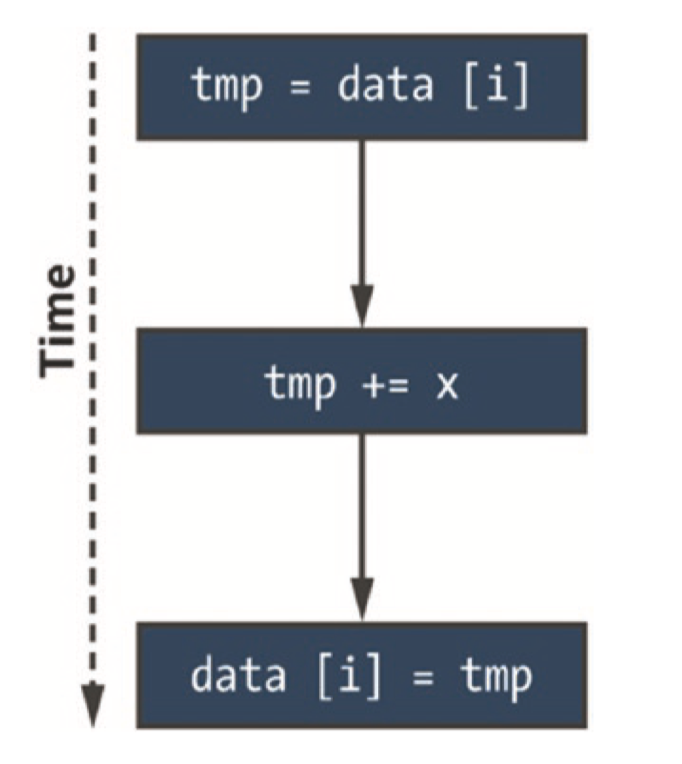
\includegraphics[width=0.9\textwidth]{figs/F19.1.png}
	\caption{\textit{数据的顺序执行[i] += x 分为三个单独的操作 }}
\end{figure}

这不是我们在开发顺序应用程序时需要担心的事情——加法的三个阶段将按照我们期望的顺序执行,如图 19-1 所示。

\begin{figure}[H]
	\centering
	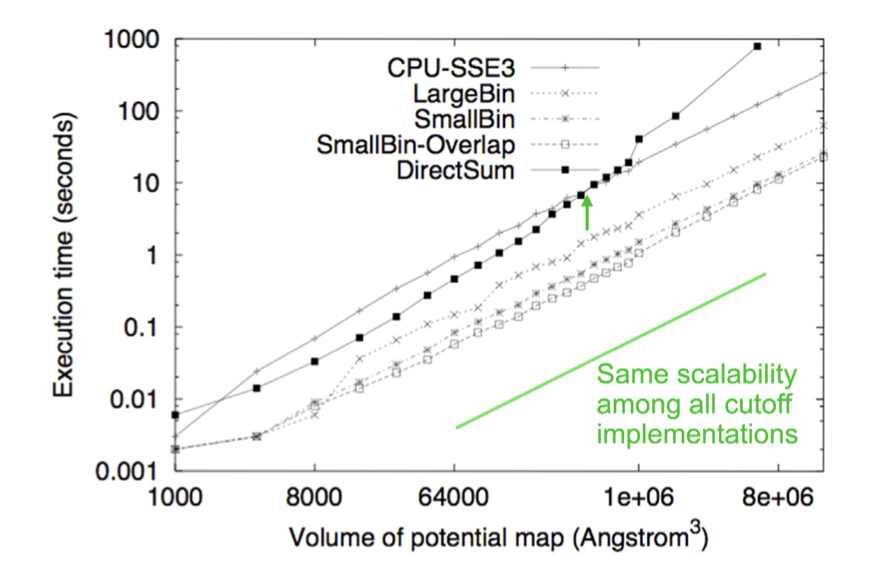
\includegraphics[width=0.9\textwidth]{figs/F19.2.png}
	\caption{\textit{一种可能的数据交错[i] += x 同时执行 }}
\end{figure}

切换到并行应用程序开发会带来额外的复杂性:如果我们同时将多个操作应用于同一数据,
我们如何确定他们对该数据的看法是一致的? 考虑图 19-2 中所示的情况,
其中 data[i] += x 的两次执行在两个线程上交错执行。 如果两个线程使用不同的 i 值,应用程序将正确执行。 
如果它们使用相同的 i 值,则两者都会从内存中加载相同的值,并且其中一个结果会被另一个结果覆盖!
 这只是调度操作的多种方式之一,我们的应用程序的行为取决于哪个线程首先获取哪个数据——我们的应用程序包含数据竞争。
 
 \begin{figure}[H]
	\centering
	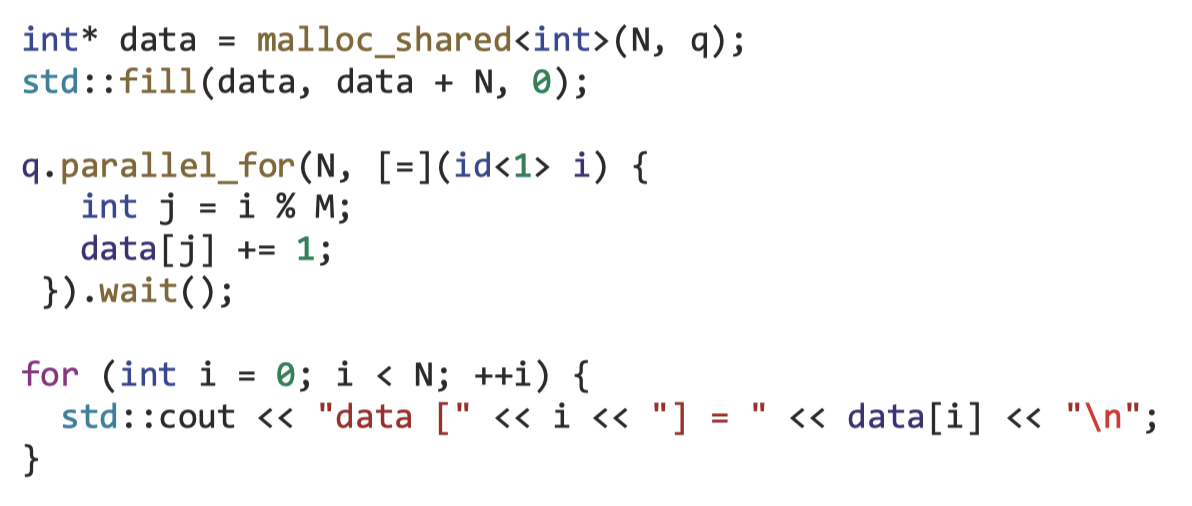
\includegraphics[width=0.9\textwidth]{figs/F19.3.png}
	\caption{\textit{包含数据争用的内核 }}
\end{figure}

\begin{figure}[H]
	\centering
	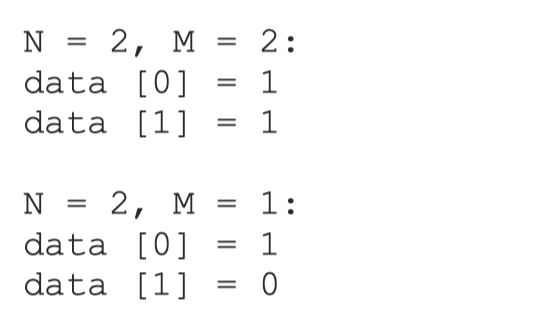
\includegraphics[width=0.9\textwidth]{figs/F19.4.png}
	\caption{\textit{图 19-3 中 N 和 M 小值的代码输出示例 }}
\end{figure}

图 19-3 中的代码及其图 19-4 中的输出显示了这种情况在实践中是多么容易发生。 
如果M大于等于N,则每个线程使用的j的值是唯一的; 如果不是,j 的值将发生冲突,并且更新可能会丢失。 
我们说可能会丢失,因为包含数据竞争的程序仍然可以在某些或一直产生正确的答案(取决于实现和硬件如何安排工作)。 
编译器和硬件都不可能知道这个程序打算做什么,或者运行时 N 和 M 的值可能是什么——作为程序员,
我们有责任了解我们的程序是否可能包含数据竞争以及它们是否对数据竞争敏感。 执行顺序。

一般来说,在开发大规模并行 SYCL 应用程序时,我们不应该关心各个Work-Items执行的确切顺序 
- 每个Kernel中希望有数百(或数千!)Work-Items,并试图强加 对它们的特定排序将对可扩展性和性能产生负面影响。 
相反,我们的重点应该是开发正确执行的可移植应用程序,
我们可以通过向编译器(和硬件)提供有关Work-Items何时共享数据、
共享发生时需要什么保证以及哪些执行顺序合法的信息来实现这一点。

\begin{remark}
	大规模并行应用程序不应关注单个工作项执行的确切顺序!
\end{remark}

\subsubsection{Barrier和栅栏}
\begin{figure}[H]
	\centering
	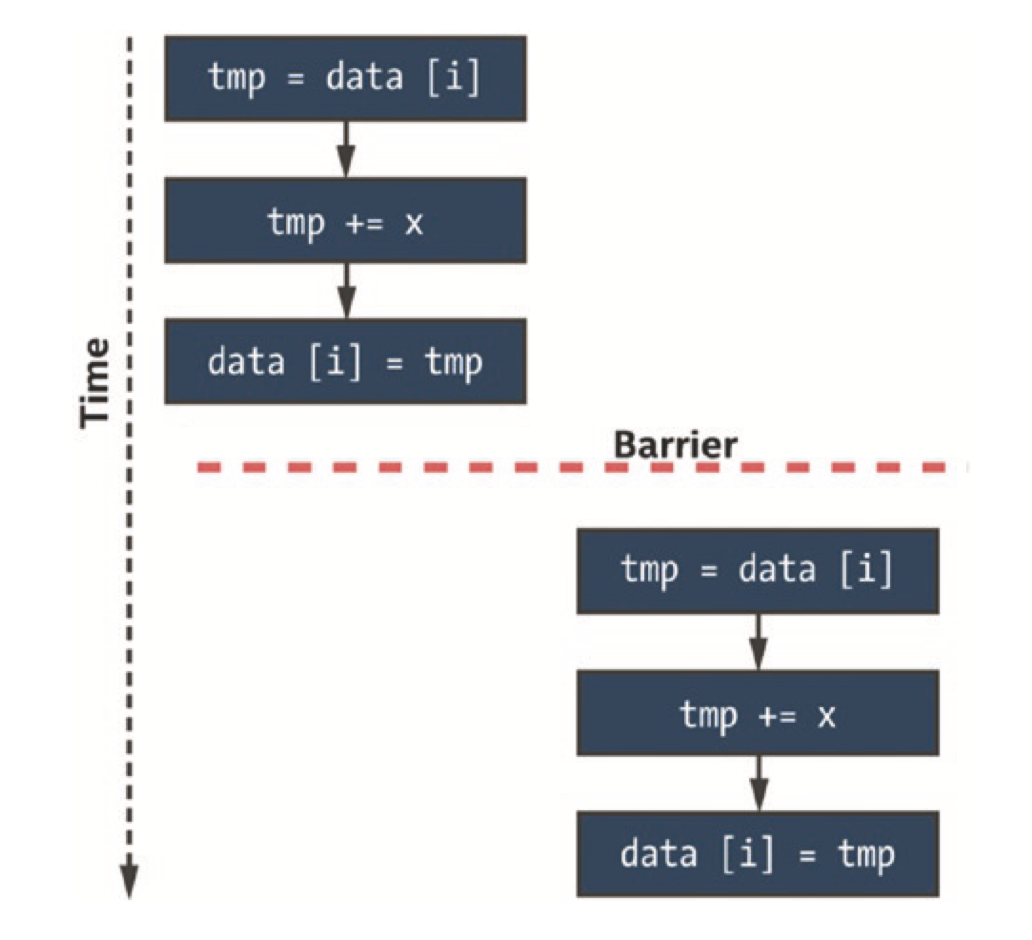
\includegraphics[width=0.9\textwidth]{figs/F19.5.png}
	\caption{\textit{两次数据执行[i] += x 由Barrier隔开 }}
\end{figure}

\begin{figure}[H]
	\centering
	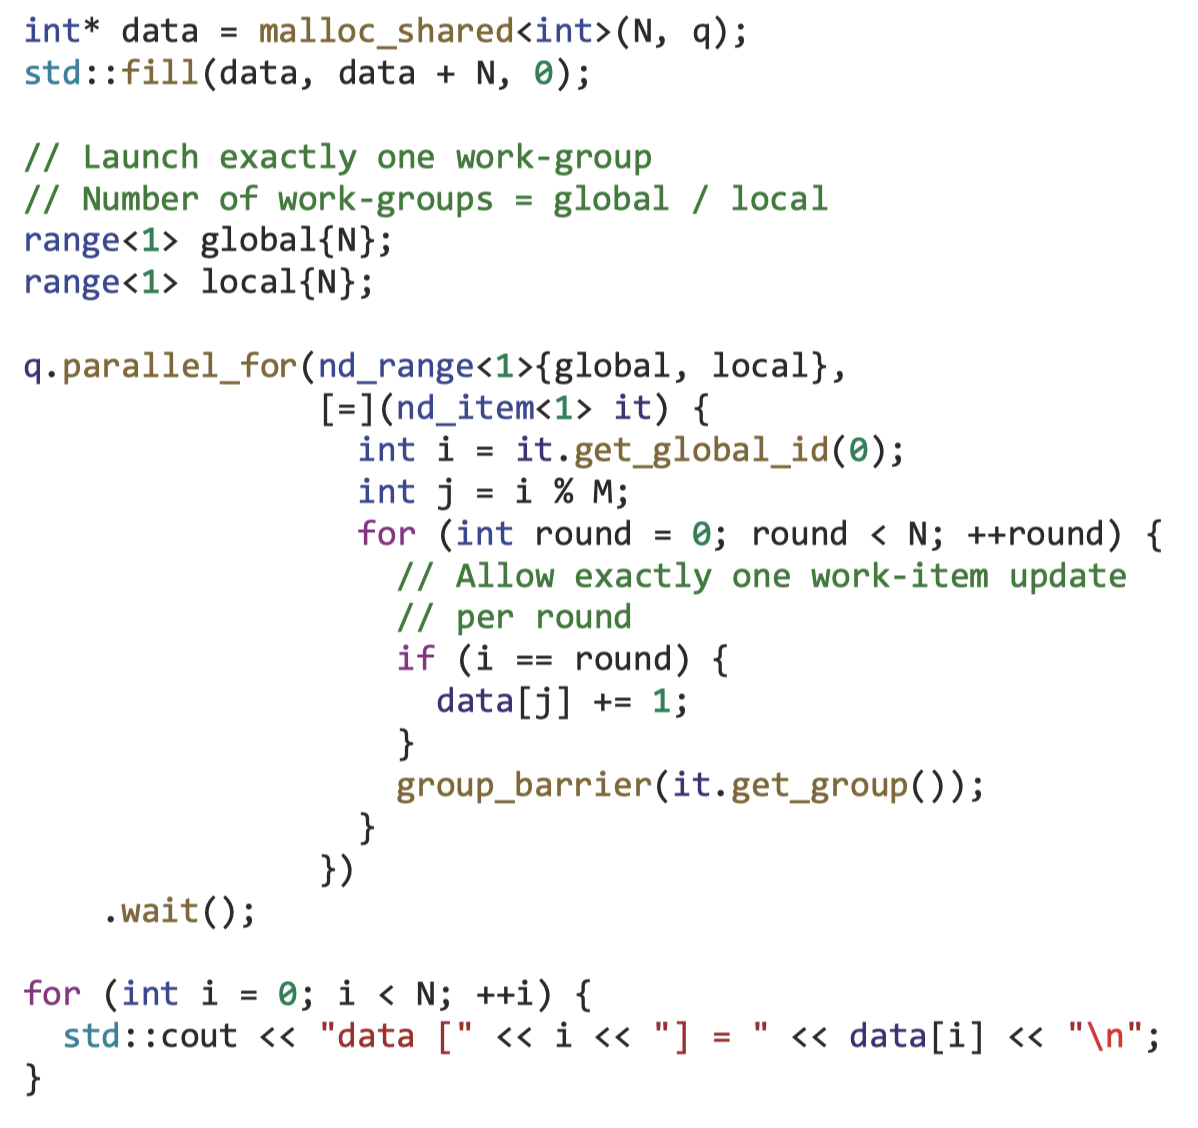
\includegraphics[width=0.9\textwidth]{figs/F19.6.png}
	\caption{\textit{使用Barrier 避免进行数据争用 }}
\end{figure}

防止同一组中的Work-Items之间发生数据争用的一种方法是使用Work-Groups Barrier和适当的内存栅栏在不同线程之间引入同步。 
我们可以使用Work-Groups Barrier来排序 data[i] 的更新,如图 19-5 所示,并且图 19-6 中给出了示例Kernel的更新版本。 
请注意,由于Work-Groups Barrier不会同步不同组中的Work-Items,
因此只有当我们将自己限制为单个Work-Groups时,我们的简单示例才能保证正确执行!

尽管使用Barrier来实现此模式是可能的,但通常不鼓励这样做 - 它强制组中的Work-Items按特定顺序顺序执行,
这可能会导致在存在负载不平衡的情况下长时间处于不活动状态。 
它还可能引入比严格必要的同步更多的同步——如果不同的Work-Items碰巧使用不同的 i 值,它们仍将被迫在Barrier处同步。

Barrier同步是一个有用的工具,可确保Work-Groups或Sub-Groups中的所有Work-Items
在进入下一阶段之前完成Kernel的某个阶段,
但对于细粒度(以及潜在的数据同步)来说过于严厉。对于更通用的同步模式,我们必须关注原子操作。

\subsubsection{原子操作}
原子操作支持对内存位置的并发访问,而不会引入数据竞争。 当多个原子操作访问同一内存时,保证它们不会重叠。 
请注意,如果只有部分访问使用原子性,则此保证不适用,并且作为程序员,
我们有责任确保我们不会使用具有不同原子性保证的操作同时访问相同的数据。

\begin{remark}
	在同一内存位置上同时混合原子和非原子操作会导致未定义的行为!
\end{remark}

\begin{figure}[H]
	\centering
	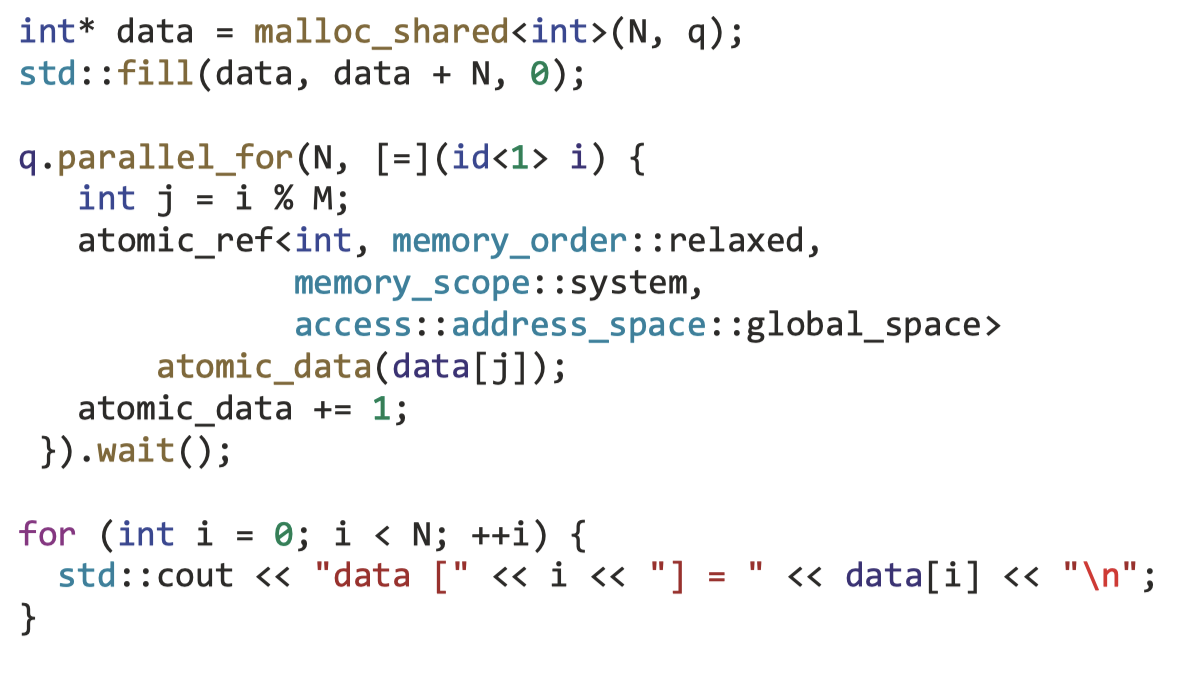
\includegraphics[width=0.9\textwidth]{figs/F19.7.png}
	\caption{\textit{使用原子操作避免进行数据竞争 }}
\end{figure}

\begin{figure}[H]
	\centering
	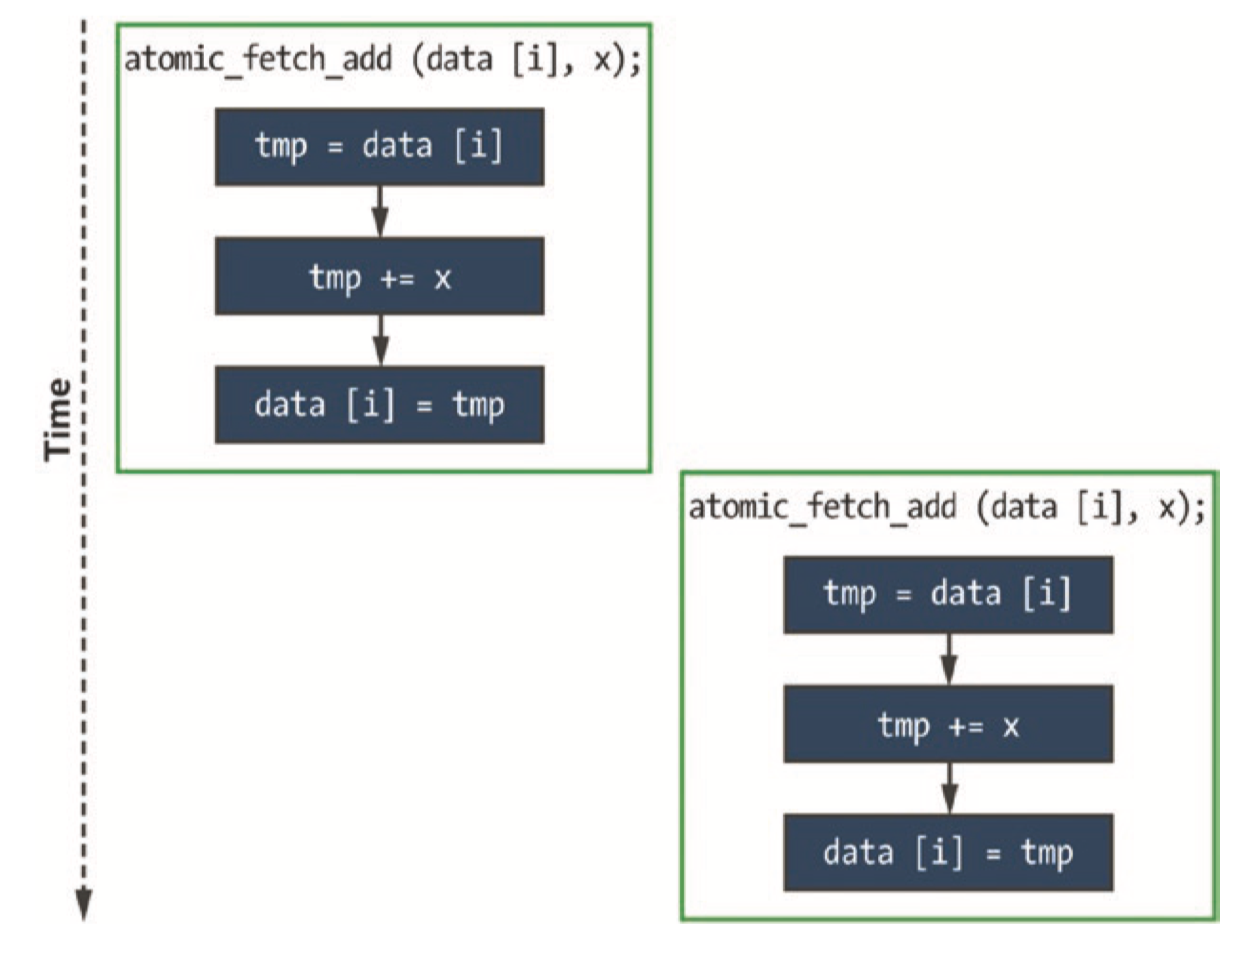
\includegraphics[width=0.9\textwidth]{figs/F19.8.png}
	\caption{\textit{与原子操作同时执行的数据交错[i] += x }}
\end{figure}

如果我们的简单加法使用原子操作来表达,结果可能如图 19-8 所示——每次更新现在都是一个不可分割的工作块,
我们的应用程序将始终产生正确的结果。 
相应的代码如图 19-7 所示——我们将在本章后面回顾atomic\_ref 类及其模板参数的含义。

然而,值得注意的是,这仍然只是一种可能的执行顺序。 
使用原子操作可以保证两个更新不会重叠(如果两个线程使用相同的 i 值),但仍然无法保证两个线程中的哪一个将首先执行。 
更重要的是,无法保证这些原子操作相对于不同线程中的任何非原子操作的排序方式。

\subsubsection{内存序}
即使在顺序应用程序中,优化编译器和硬件也可以自由地重新排序操作,如果它们不改变应用程序的可观察行为。 
换句话说,应用程序的行为必须完全按照程序员编写的方式运行。

不幸的是,这种假设的保证不足以帮助我们推理并行程序的执行。 
我们现在需要担心两个重新排序的来源:编译器和硬件可能会对每个顺序线程内的语句执行重新排序,
并且线程本身可以以任何(可能是交错的)顺序执行。 
为了设计和实现线程之间的安全通信协议,我们需要能够限制这种重新排序。 
通过向编译器提供有关我们所需的内存顺序的信息,我们可以防止与应用程序的预期行为不兼容的重新排序优化。

三种常用的内存顺序是:

\begin{enumerate}
	\item 宽松的内存排序

	\item 获取-释放或释放-获取内存顺序

	\item 顺序一致的内存排序
\end{enumerate}

在宽松的内存排序下,内存操作可以不受任何限制地重新排序。 
宽松内存模型最常见的用法是递增共享变量(例如,单个计数器、直方图计算期间的值数组)。

在获取-释放内存顺序下,一个线程释放一个原子变量,另一个线程获取相同的原子变量,充当这两个线程之间的同步点,
并保证释放线程发出的任何先前对内存的写入对于获取线程都是可见的 。 
通俗地说,我们可以认为原子操作将其他内存操作的副作用释放到其他线程,或者获取其他线程上的内存操作的副作用。 
如果我们想通过内存在线程对之间传递值,则需要这样的内存模型,这可能比我们想象的更常见。 
当程序获取锁时,它通常会继续执行一些额外的计算并在最终释放锁之前修改一些内存 - 只有锁变量会被原子更新,
但我们希望受锁保护的内存更新能够免受数据竞争的影响 。 
此行为依赖于获取-释放内存顺序的正确性,并且尝试使用宽松的内存顺序来实现锁将不起作用。

在顺序一致的内存排序下,获取-释放顺序的保证仍然有效,但还存在所有原子操作的单个全局顺序。 
这种内存排序的行为是三者中最直观的,也是最接近我们在开发顺序应用程序时习惯依赖的原始假设保证的。 
通过顺序一致性,推理线程组(而不是线程对)之间的通信变得更加容易,
因为所有线程必须就所有原子操作的全局顺序达成一致。

了解编程模型和设备的组合支持哪些内存顺序是设计可移植并行应用程序的必要部分。 
明确地描述应用程序所需的内存顺序可确保当我们所需的行为不受支持时,
应用程序可以预见地失败(例如,在编译时),并防止我们做出不安全的假设。

\subsection{内存模型}
到目前为止,本章已经介绍了理解内存模型所需的概念。 本章的其余部分详细解释了内存模型,包括

\begin{itemize}
	\item 如何表达Kernel的内存排序要求

	\item 如何查询特定设备支持的内存顺序

	\item 内存模型在不相交的地址空间和多个设备方面的行为方式

	\item 内存模型如何与Barrier、栅栏和原子交互

	\item Buffer和 USM 之间使用原子操作有何不同
\end{itemize}

该内存模型基于 C++ 的内存模型,但在一些重要方面有所不同。 
这些差异反映了我们的长期愿景,即 SYCL 应该帮助告知 C++ 的未来:类的默认行为和命名与 C++ 标准库紧密一致,
旨在扩展 C++ 功能而不是限制它。

图 19-9 中的表总结了 C++(C++11、C++14、C++17、C++20)与 SYCL 中如何将不同的内存模型概念公开为语言功能。 
C++14、C++17 和 C++20 标准还包含一些影响 C++ 实现的说明。 
这些说明不应影响我们编写的应用程序代码,因此我们在此不讨论它们。

\begin{figure}[H]
	\centering
	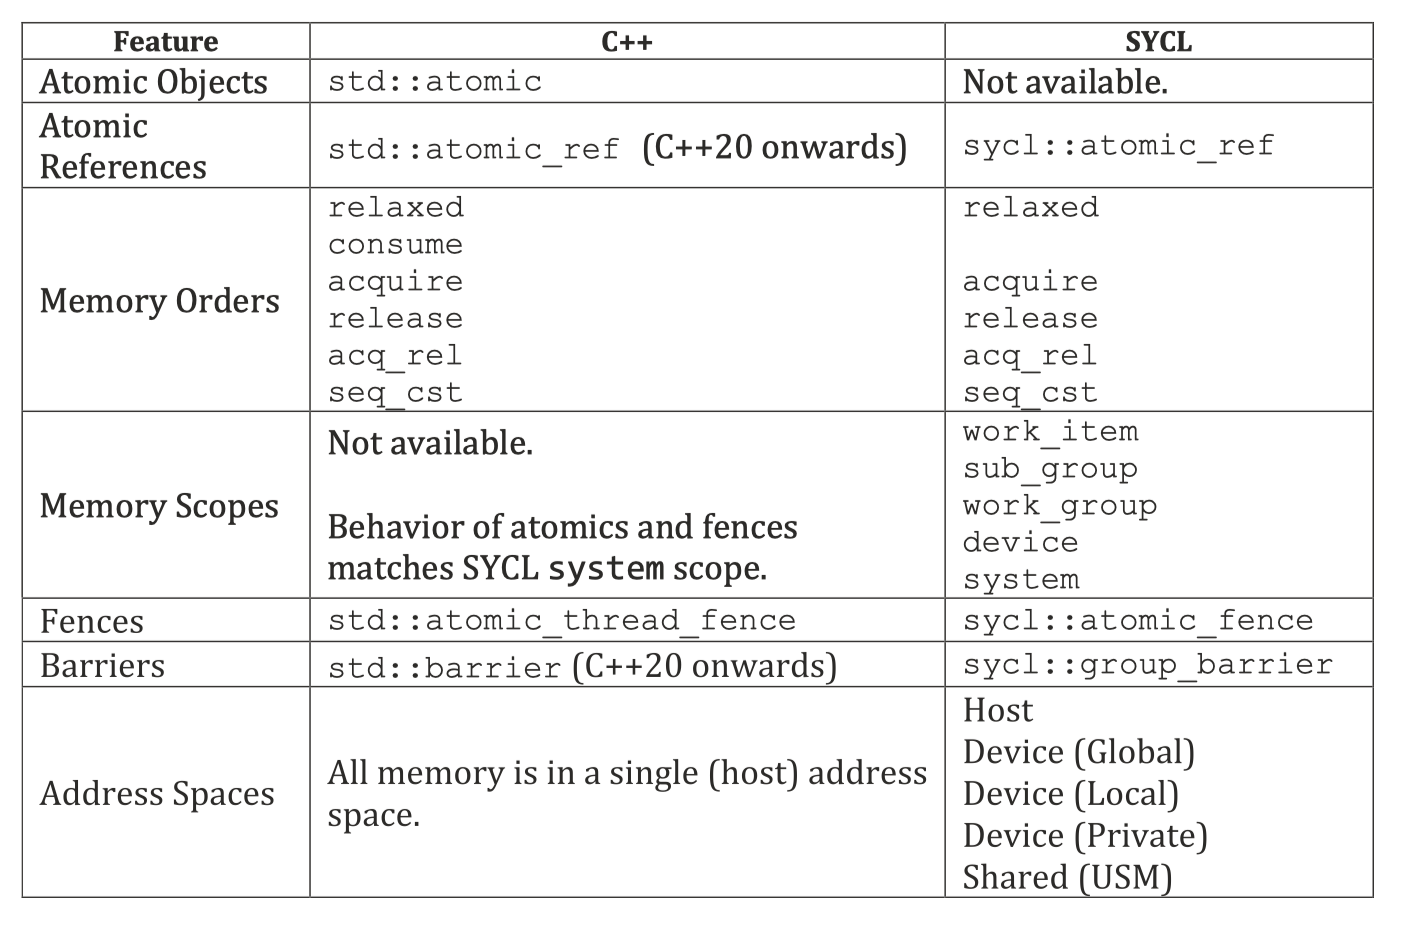
\includegraphics[width=0.9\textwidth]{figs/F19.9.png}
	\caption{\textit{比较 C++ 和 SYCL 内存模型 }}
\end{figure}

\subsubsection{memory\_order枚举类}
内存模型通过 memory\_order 枚举类的五个值公开不同的内存顺序(注意:C++“consume”不是 SYCL 的一部分),
这些值可以作为参数提供给栅栏和原子操作。 
向操作提供内存顺序参数告诉编译器相对于该操作的所有其他内存操作(到任何地址)需要什么内存顺序保证,如下所述:

\begin{itemize}
	\item memory\_order::relaxed 读写操作可以在操作之前或之后重新排序,没有任何限制,没有序保证。

	\item memory\_order::acquire 程序中在该操作之后出现的读和写操作必须在该操作之后出现
	(即,它们不能在该操作之前重新排序)。

	\item memory\_order::release 程序中出现在该操作之前的读写操作必须发生在该操作之前
	(即操作之后不能重新排序),并且保证前面的写操作对已同步的其他Work-Items可见 通过相应的获取操作
	(即使用相同变量和 memory\_order::acquire 或Barrier函数的原子操作)。

	\item memory\_order::acq\_rel 该操作既充当获取又充当释放。 
	读取和写入操作不能围绕该操作重新排序,并且前面的写入必须可见,如之前针对 memory\_order::release 所描述的。

	\item memory\_order::seq\_cst 该操作分别充当获取、释放或两者,具体取决于它是读、写还是读-修改-写操作。 
	具有此内存顺序的所有操作都以连续一致的顺序观察。
\end{itemize}

\begin{figure}[H]
	\centering
	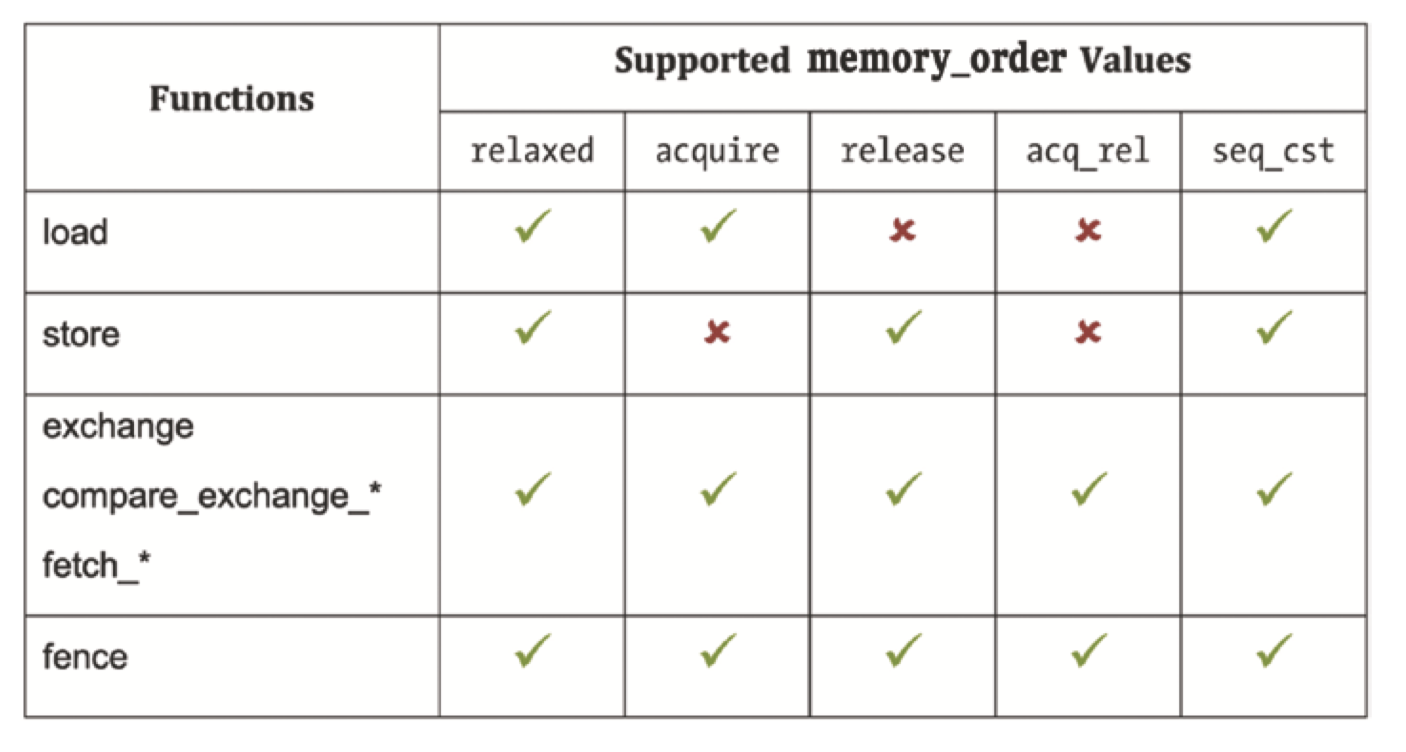
\includegraphics[width=0.9\textwidth]{figs/F19.10.png}
	\caption{\textit{支持原子操作memory\_order }}
\end{figure}

每个操作支持哪些内存顺序有几个限制。 图 19-10 中的表总结了哪些组合是有效的。

加载操作不会将值写入内存,因此与释放语义不兼容。 类似地,存储操作不会从内存中读取值,因此与获取语义不兼容。 
其余的读-修改-写原子操作和栅栏与所有内存顺序兼容。

\begin{remark}[C++ 中的内存序]
	C++内存模型还包括 memory\_order::consume,其行为与 memory\_order::acquire 类似。
	但是,C++17不鼓励使用它,并指出其定义正在修订中。因此,将其纳入 SYCL 有待考虑用于未来的规范。
\end{remark}

\subsubsection{memory\_scope 枚举类}
C++ 内存模型假设应用程序在具有单个地址空间的单个设备上执行。 
这些假设均不适用于 SYCL 应用程序:应用程序的各个部分在不同的设备(即主机和一个或多个加速器设备)上执行; 
每个设备都有多个地址空间(即私有、本地和全局); 
每个设备的全局地址空间可能不相交,也可能不相交(取决于 USM 支持)。

为了解决这个问题,SYCL 扩展了内存顺序的 C++ 概念,以包含原子操作的范围,表示给定内存顺序约束适用的最小Work-Items集。 
这组范围是通过 memory\_scope 枚举类来定义的:

\begin{itemize}
	\item memory\_scope::work\_item

内存排序约束仅适用于调用Work-Items。 此范围仅对图像操作有用,因为Work-Items内的所有其他操作都已保证按程序顺序执行。

	\item memory\_scope::sub\_group, memory\_scope::work\_group

内存排序约束仅适用于与调用Work-Items位于同一Sub-Groups或Work-Groups中的Work-Items。

	\item memory\_scope::device

内存排序约束仅适用于与调用Work-Items在同一设备上执行的Work-Items。

	\item memory\_scope::system

内存排序约束适用于系统中的所有Work-Items。
\end{itemize}

除非设备功能施加限制,否则所有内存范围都是所有原子和栅栏操作的有效参数。 
但是,在以下三种情况之一中,范围参数可能会自动降级为更窄的范围:

\begin{enumerate}
	\item 如果原子操作更新Work-Groups本地内存中的值,
	则任何比 memory\_scope::work\_group 更宽的范围都会缩小(因为本地内存仅对同一Work-Groups中的Work-Items可见)。

	\item 如果设备不支持USM,则指定memory\_scope::system 
	始终等同于memory\_scope::device(因为多个设备不能同时访问Buffer)。

	\item 如果原子操作使用 memory\_order::relaxed,则没有顺序保证,
	并且内存范围参数实际上被忽略。
\end{enumerate}

\subsubsection{查询设备能力}
为了确保与早期版本 SYCL 支持的设备兼容并最大限度地提高可移植性,
SYCL 支持 OpenCL 1.2 设备和其他可能无法支持完整 C++ 内存模型的硬件(例如某些类别的嵌入式设备)。 
SYCL 提供设备查询来帮助我们推断系统中可用设备支持的内存顺序和内存范围:

\begin{itemize}
	\item atomic\_memory\_order\_capabilities

	返回特定设备上原子操作支持的所有内存排序的列表。

	所有设备都必须至少支持 memory\_order::relaxed。

	\item atomic\_fence\_order\_capabilities

	返回特定设备上的栅栏操作支持的所有内存排序的列表。

	所有设备都必须至少支持memory\_order::relaxed、memory\_order::acquire、memory\_order::release 
	和memory\_order::acq\_rel。 请注意,栅栏的最低要求强于原子操作的最低要求,
	因为此类栅栏对于在存在Barrier的情况下推理内存顺序至关重要。

	\item atomic\_memory\_scope\_capabilities

	atomic\_fence\_scope\_capabilities

	返回特定设备上原子和栅栏操作支持的所有内存范围的列表。 所有设备都必须至少支持 memory\_order::work\_group。
\end{itemize}

一开始可能很难记住哪些功能和设备功能的组合支持哪些内存顺序和范围。 
在实践中,我们可以通过遵循下面概述的两种开发方法之一来避免这种复杂性:
\begin{enumerate}
	\item 开发具有顺序一致性和系统围栏的应用程序。

	在性能调优期间仅考虑采用不太严格的内存顺序。

	\item 开发具有宽松一致性和Work-Groups界限的应用程序。

	仅在需要正确性时才考虑采用更严格的内存顺序和更广泛的内存范围。
\end{enumerate}

第一种方法确保所有原子操作和栅栏的语义与 C++ 的默认行为相匹配。 
这是最简单且最不易出错的选项,但性能和可移植性特征最差。

第二种方法更符合以前版本的 SYCL 和 OpenCL 等语言的默认行为。 
尽管更复杂(因为它要求我们更加熟悉不同的内存顺序和范围),
但它确保我们编写的大部分 SYCL 代码都可以在任何设备上运行,而不会造成性能损失。

\subsubsection{Barrier和栅栏}
到目前为止,本书中所有之前对Barrier和栅栏的使用都依赖于默认行为,忽略了内存顺序和范围的问题。

默认情况下,SYCL 中的每个组Barrier充当调用Work-Items可访问的所有地址空间的获取-释放栅栏,
并使先前的写入至少对同一组中的所有其他Work-Items可见(由组的 fence\_scope 定义) 成员变量)。 
这确保了Barrier后一组Work-Items内的内存一致性,符合我们对同步含义的直觉(以及 C++ 中同步关系的定义)。 
可以通过将显式的 Memory\_scope 参数传递给 group\_Barrier 函数来覆盖此默认行为。

atomic\_fence 函数为我们提供了比这更细粒度的控制,允许Work-Items执行指定内存顺序和范围的栅栏。

\subsubsection{SYCL 中的原子操作}
SYCL 提供对多种数据类型的多种原子操作的支持。 
所有设备都保证支持常见操作的原子版本(例如加载、存储、算术运算符),以及实现无锁算法所需的原子比较和交换操作。 
该语言为所有基本整数、浮点和指针类型定义了这些操作 - 所有设备都必须支持 32 位类型的这些操作,
但 64 位类型支持是可选的。

\paragraph{atomic 类}

C++11 中的 std::atomic 类提供了用于创建和操作原子变量的接口。 
原子类的实例拥有自己的数据,不能移动或复制,只能使用原子操作进行更新。 
这些限制显着减少了错误使用类和引入未定义行为的机会。 
不幸的是,它们还阻止该类在 SYCL Kernel中使用——不可能在主机上创建原子对象并将它们传输到设备! 
我们可以继续在主机代码中使用 std::atomic,但尝试在设备Kernel中使用它会导致编译器错误。

\begin{remark}[SYCL 2020 中不推荐使用的原子类]
SYCL 1.2.1 规范包括一个 cl::sycl::atomic 类,
该类松散地基于 C++ 11 中的 std::atomic 类。我们之所以这么说,是因为这两个类的接口之间存在一些差异,
最明显的是 SYCL 1.2.1 版本不拥有其数据,并且默认为宽松的内存排序。
\end{remark}

cl::sycl::atomic 类在 SYCL 2020 中已弃用。应使用 atomic\_ref 类(在下一节中介绍)来代替它。

\paragraph{atomic\_ref 类}

C++20 中的 std::atomic\_ref 类为原子操作提供了一个替代接口,它比 std::atomic 提供了更大的灵活性。 
这两个类之间最大的区别是 std::atomic\_ref 的实例不拥有其数据,而是从现有的非原子变量构造而成。 
创建原子引用有效地充当了一个承诺,即仅在引用的生命周期内以原子方式访问引用的变量。 
这些正是 SYCL 所需的语义,因为它们允许我们在主机上创建非原子数据,
将该数据传输到设备,并仅在传输后将其视为原子数据。 
因此,SYCL Kernel中使用的atomic\_ref 类基于std::atomic\_ref。

\begin{figure}[H]
	\centering
	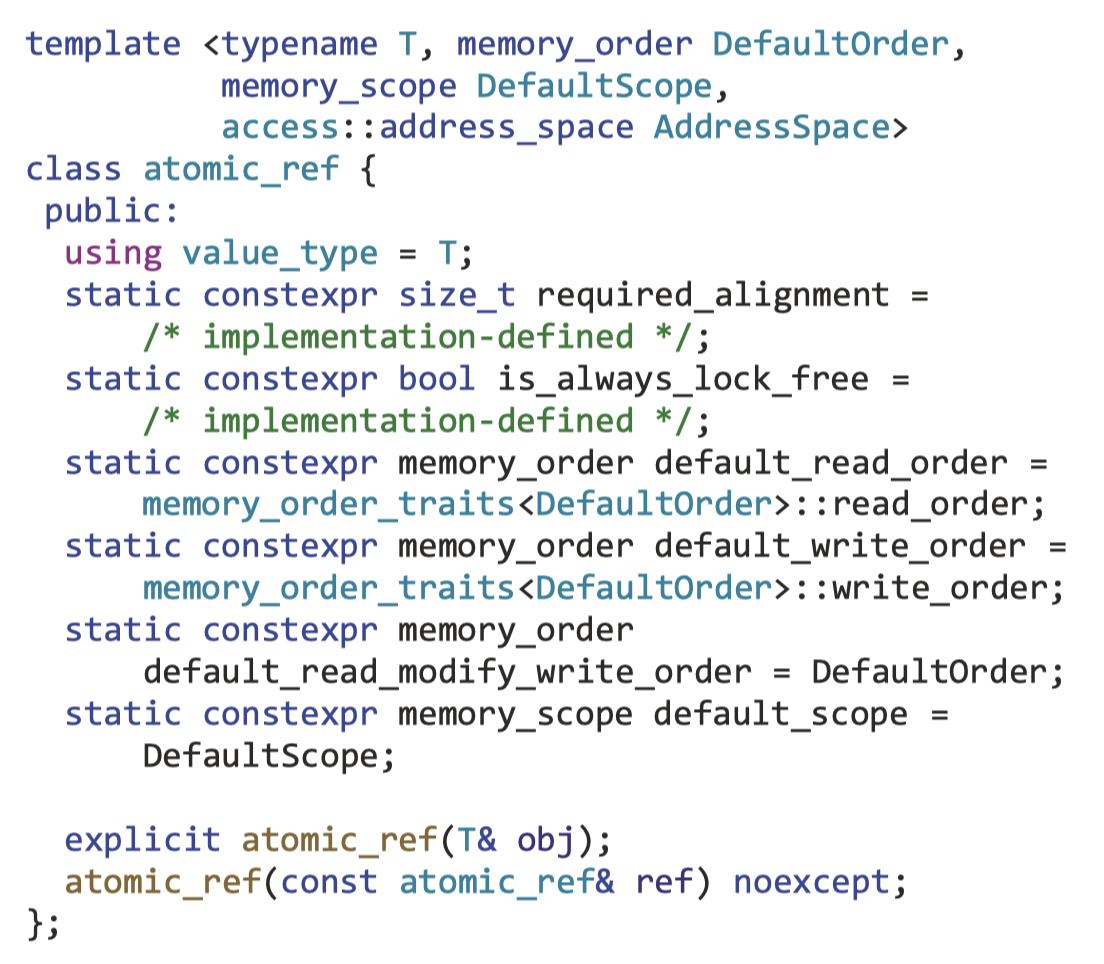
\includegraphics[width=0.9\textwidth]{figs/F19.11.png}
	\caption{\textit{atomic\_ref 类的构造函数和静态成员 }}
\end{figure}

我们说基于是因为该类的 SYCL 版本包括三个附加模板参数,如图 19-11 所示。

如前所述,不同 SYCL 设备的功能各不相同。 
为 SYCL 的原子类选择默认行为是一个困难的提议:
默认为 C++ 行为(即 memory\_order::seq\_cst、memory\_scope::system)会限制代码仅在功能最强大的设备上执行; 
另一方面,在迁移现有 C++ 代码时,
打破 C++ 约定并默认使用最低公分母(即 memory\_order::relaxed、memory\_scope::work\_group)
可能会导致意外行为。 
SYCL 采用的设计提供了一种折衷方案,允许我们将所需的默认行为定义为对象类型的一部分
(使用 DefaultOrder 和 DefaultScope 模板参数)。 
其他顺序和范围可以作为我们认为合适的特定原子操作的运行时参数提供
 - DefaultOrder 和 DefaultScope 仅影响我们不或无法覆盖默认行为的操作
 (例如,当使用像 += 这样的速记运算符时)。 最后一个(可选)模板参数表示分配引用对象的地址空间。 
 请注意,如果未指定最终模板参数,则引用的变量可以分配在任何地址空间中 - 尽管此处指定地址空间是可选的,
 但我们建议提供显式地址空间(如果可能),以便为编译器提供更多信息并避免不需要的信息 性能开销。

原子引用根据其引用的对象类型提供对不同操作的支持。 
所有类型都支持的基本操作如图 19-12 所示,提供了原子地将数据移入和移出内存的能力。

\begin{figure}[H]
	\centering
	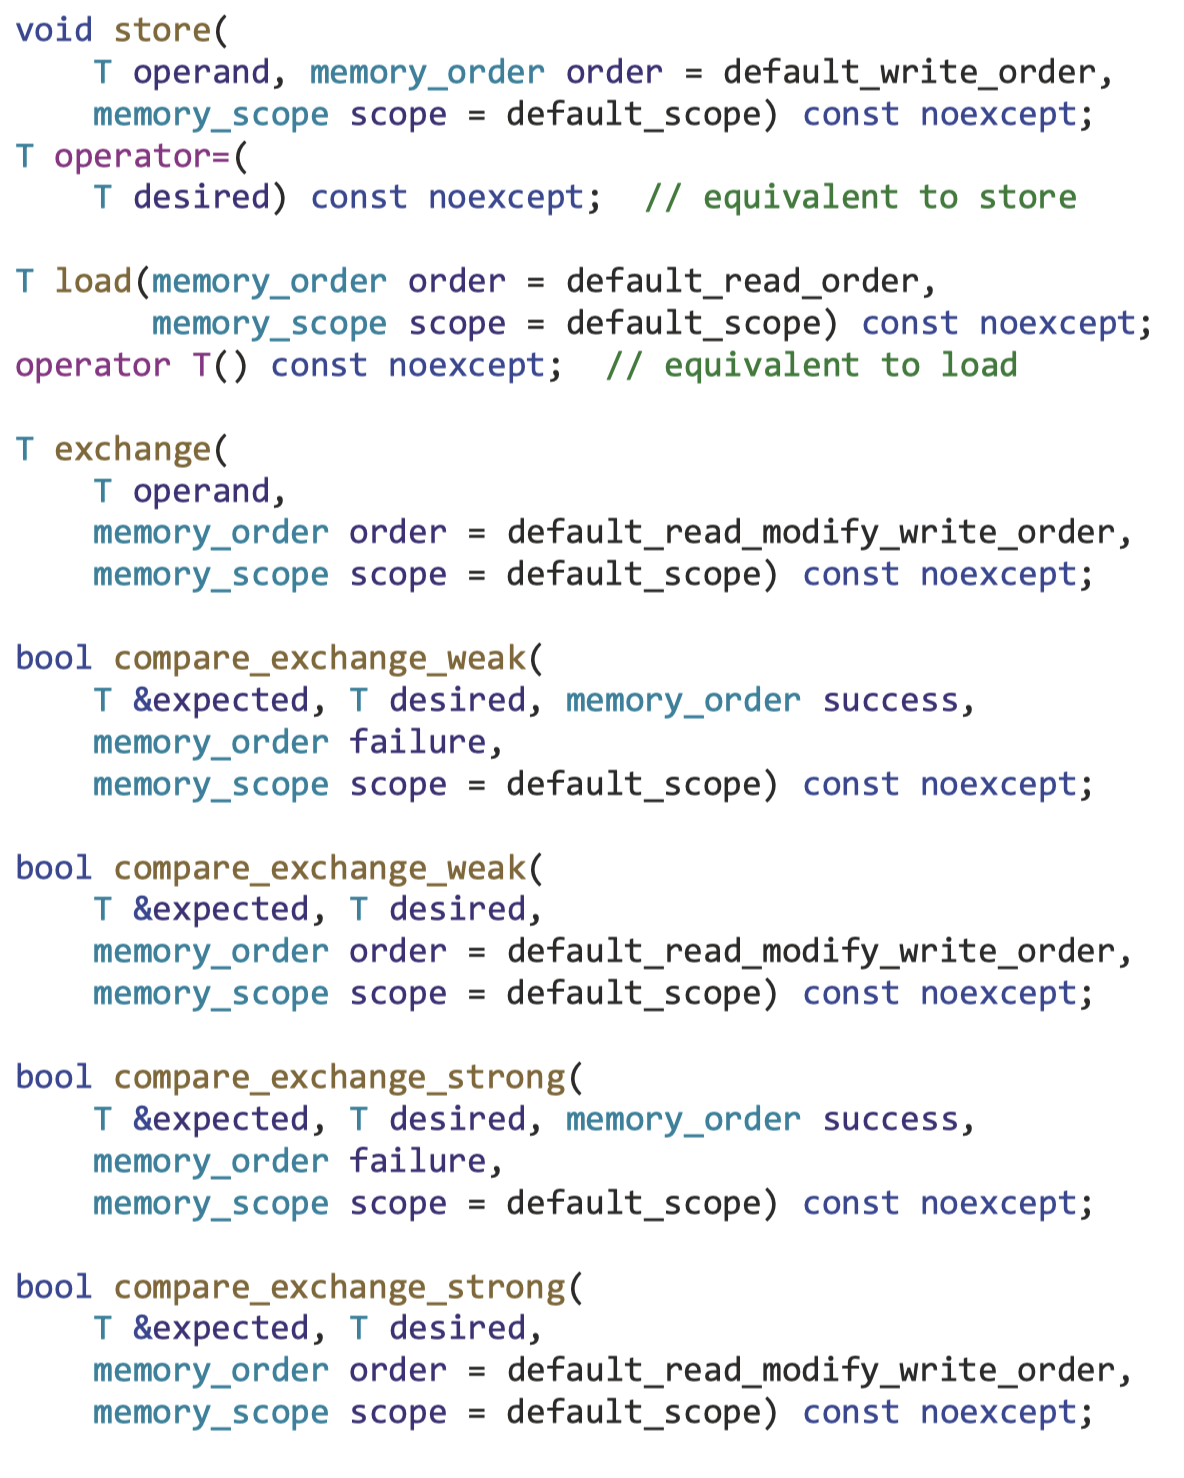
\includegraphics[width=0.9\textwidth]{figs/F19.12.png}
	\caption{\textit{所有类型的atomic\_ref的基本操作 }}
\end{figure}

\begin{figure}[H]
	\centering
	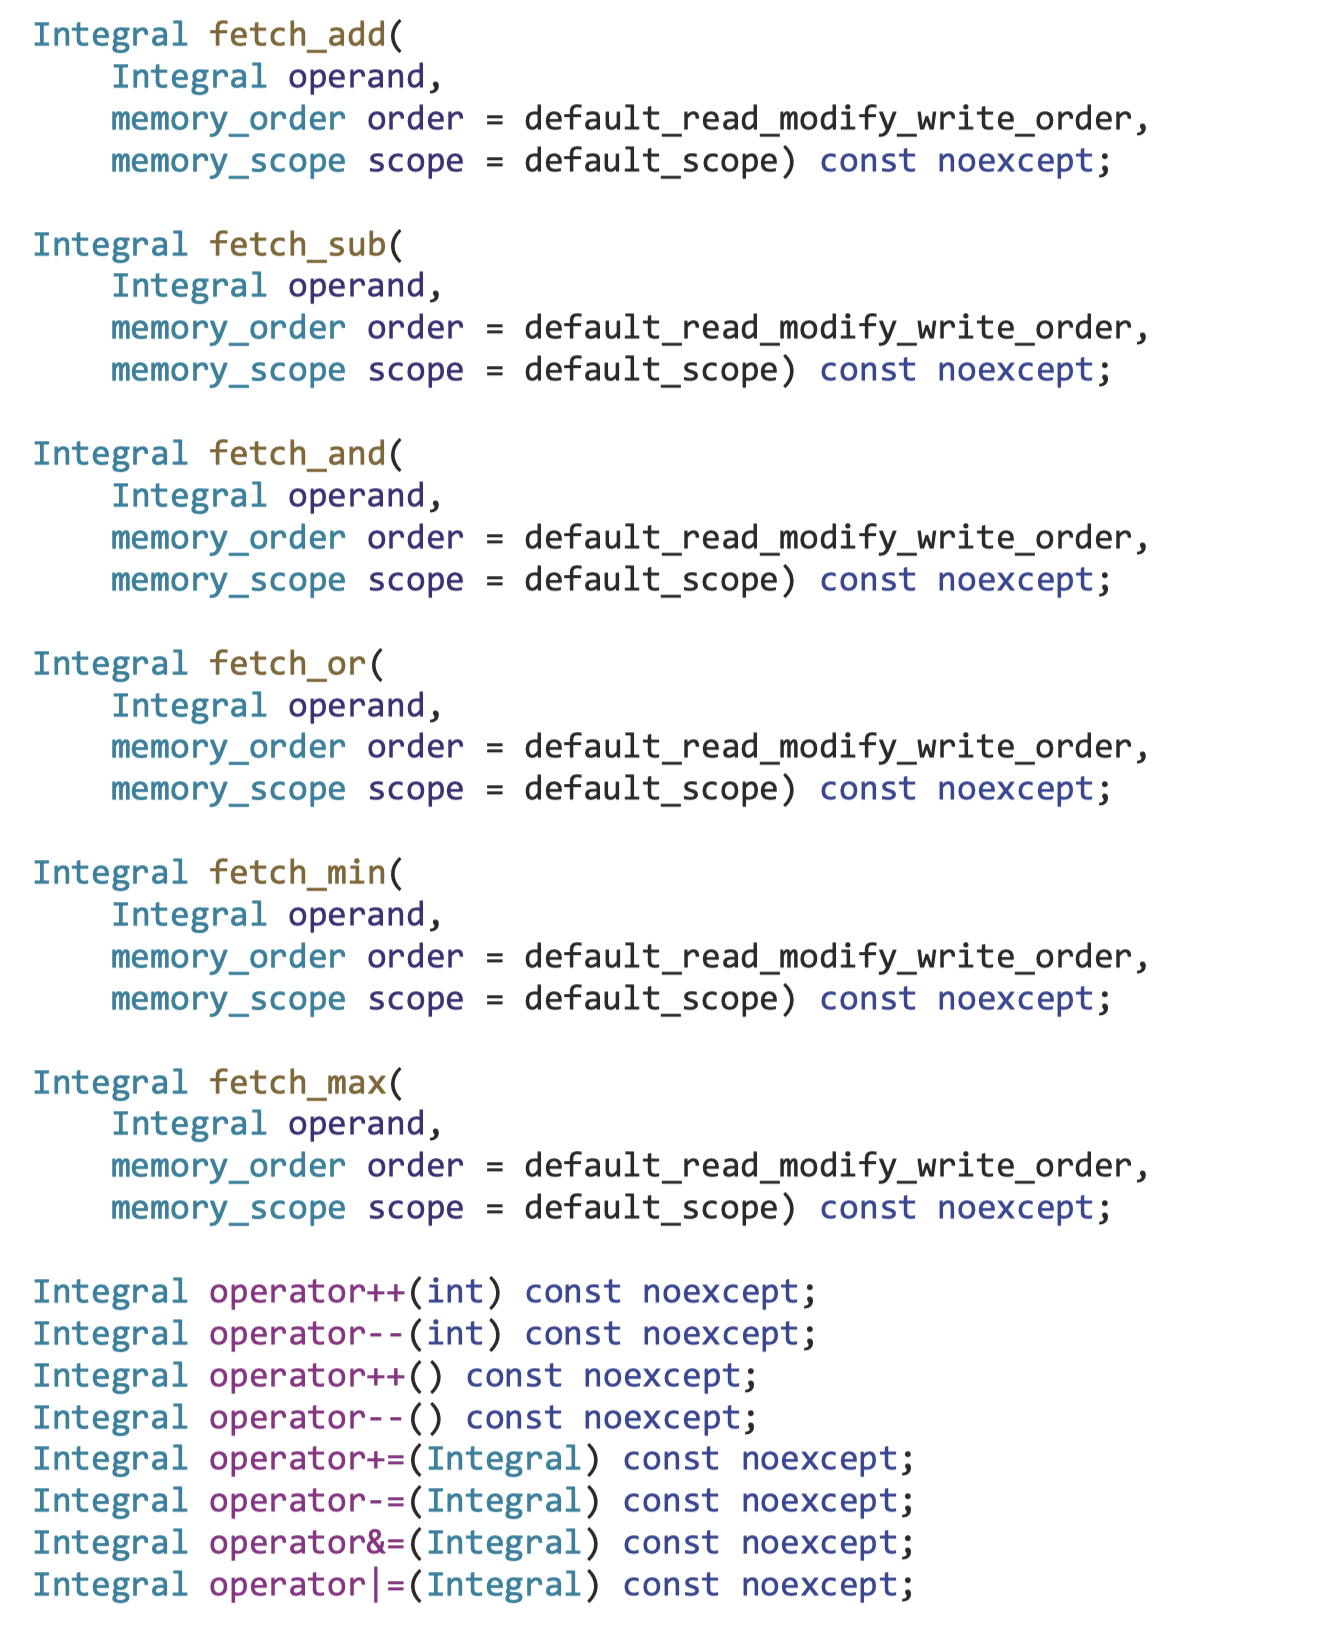
\includegraphics[width=0.9\textwidth]{figs/F19.13.png}
	\caption{\textit{仅针对整型的atomic\_ref附加操作 }}
\end{figure}

\begin{figure}[H]
	\centering
	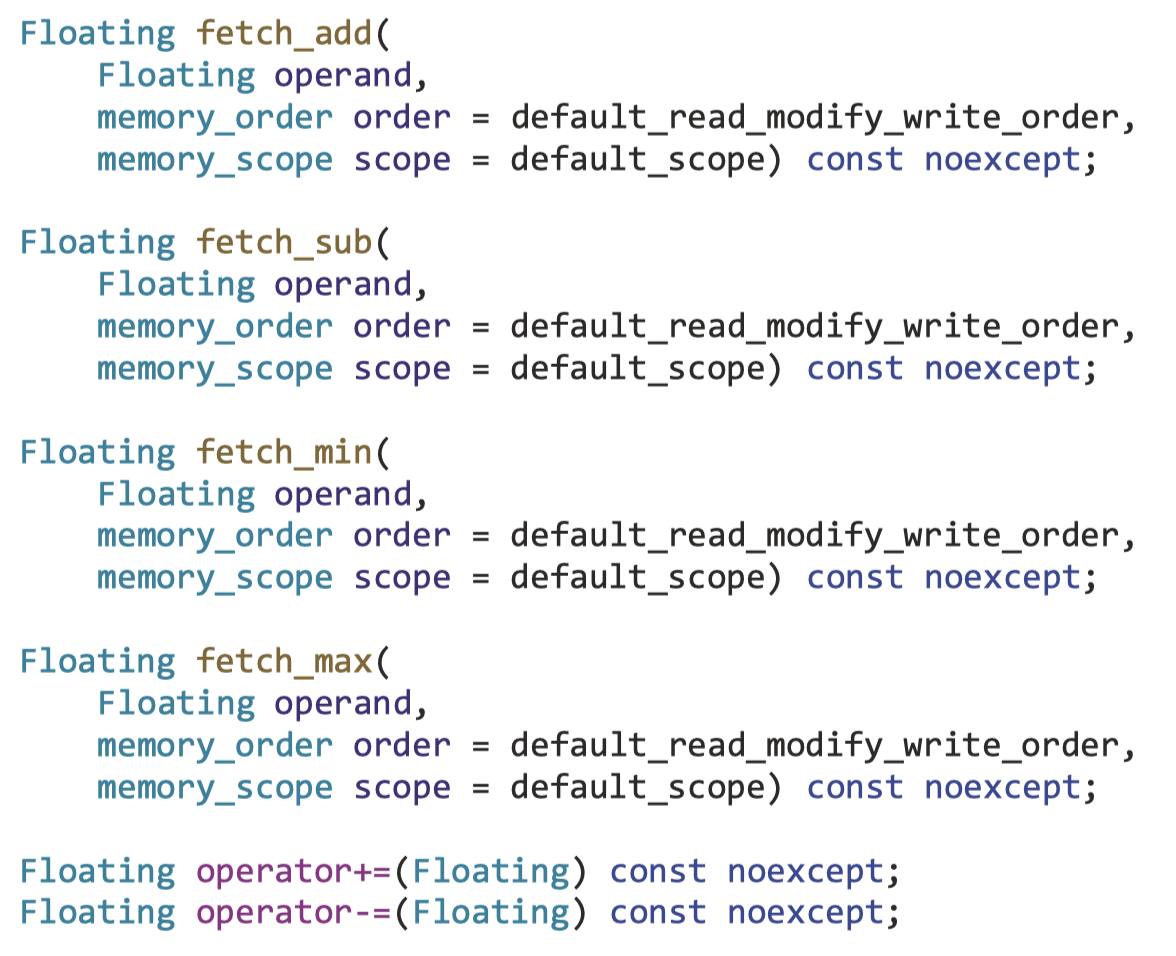
\includegraphics[width=0.9\textwidth]{figs/F19.14.png}
	\caption{\textit{仅对浮点类型进行atomic\_ref的附加操作 }}
\end{figure}

对整型和浮点类型对象的原子引用扩展了可用原子操作集以包括算术操作,如图 19-13 和图 19-14 所示。 
设备需要支持原子浮点类型,无论它们是否在硬件中具有对浮点原子的本机支持,
并且许多设备期望使用原子比较交换来模拟原子浮点加法。 
这种模拟是在 SYCL 中提供性能和可移植性的重要部分,
我们应该在算法需要的任何地方随意使用浮点原子——生成的代码将在任何地方正确工作,
并将受益于浮点原子的未来改进 硬件无需任何修改!

\subsubsection{将原子与Buffer一起使用}
正如上一节所讨论的,SYCL 中无法分配原子数据并在主机和设备之间移动它。 
要将原子操作与Buffer结合使用,我们必须创建一个要传输到设备的非原子数据Buffer,然后通过原子引用访问该数据。

\begin{figure}[H]
	\centering
	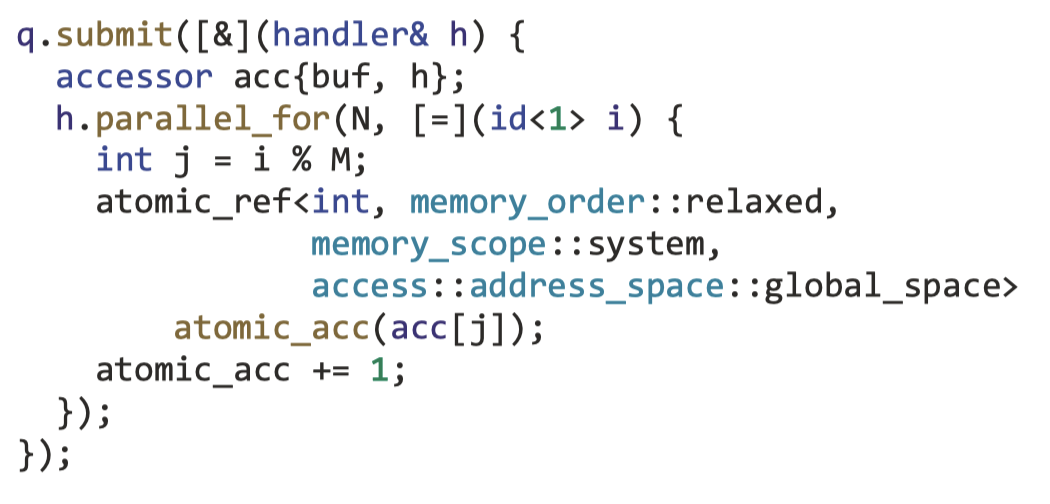
\includegraphics[width=0.9\textwidth]{figs/F19.15.png}
	\caption{\textit{通过显式创建的atomic\_ref访问Buffer }}
\end{figure}

图19-15中的代码是使用显式创建的原子引用对象在SYCL中表达原子性的示例。 
Buffer存储普通整数,我们需要一个具有读写权限的访问器。 
然后,我们可以使用 += 运算符作为 fetch\_add 成员函数的简写替代,为每个数据访问创建一个atomic\_ref 实例。

如果我们想要在同一Kernel中混合对Buffer的原子和非原子访问,以避免在不需要时支付原子操作的性能开销,则此模式非常有用。 
如果我们知道Buffer中的内存位置的子集将被多个Work-Items同时访问,则在访问该子集时只需要使用原子引用。 
或者,如果我们知道同一Work-Groups中的Work-Items仅在Kernel的一个阶段
(即两个Work-Groups Barrier之间)同时访问本地内存,
则我们只需要在该阶段使用原子引用。 
当像这样混合原子和非原子访问时,重要的是要注意对象的生命周期——虽然存在引用特定对象的任何atomic\_ref,
但对该对象的所有访问都必须通过atomic\_ref的实例(原子地)发生。

\subsubsection{将原子与统一共享内存结合使用}
\begin{figure}[H]
	\centering
	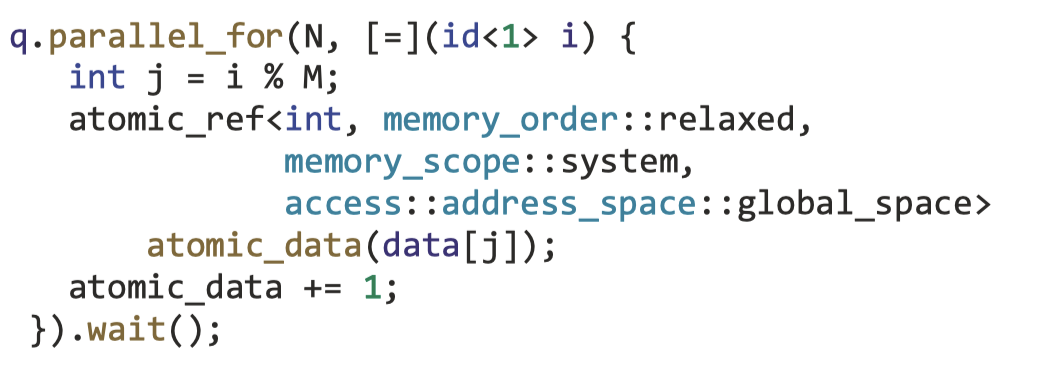
\includegraphics[width=0.9\textwidth]{figs/F19.16.png}
	\caption{\textit{通过显式创建的atomic\_ref访问 USM 分配 }}
\end{figure}

如图 19-16 所示(从图 19-7 复制),我们可以按照与Buffer完全相同的方式从 USM 中存储的数据构造原子引用。 
实际上,此代码与图 19-15 中所示的代码之间的唯一区别是 USM 代码不需要Buffer或访问器。

\subsection{在现实生活中使用原子}
原子的潜在用途是如此广泛和多样,我们不可能在本书中提供每种用途的示例。 
我们提供了两个具有跨领域广泛适用性的代表性示例:

\begin{enumerate}
	\item 计算直方图

	\item 实现全设备同步
\end{enumerate}

\subsubsection{计算直方图}
\begin{figure}[H]
	\centering
	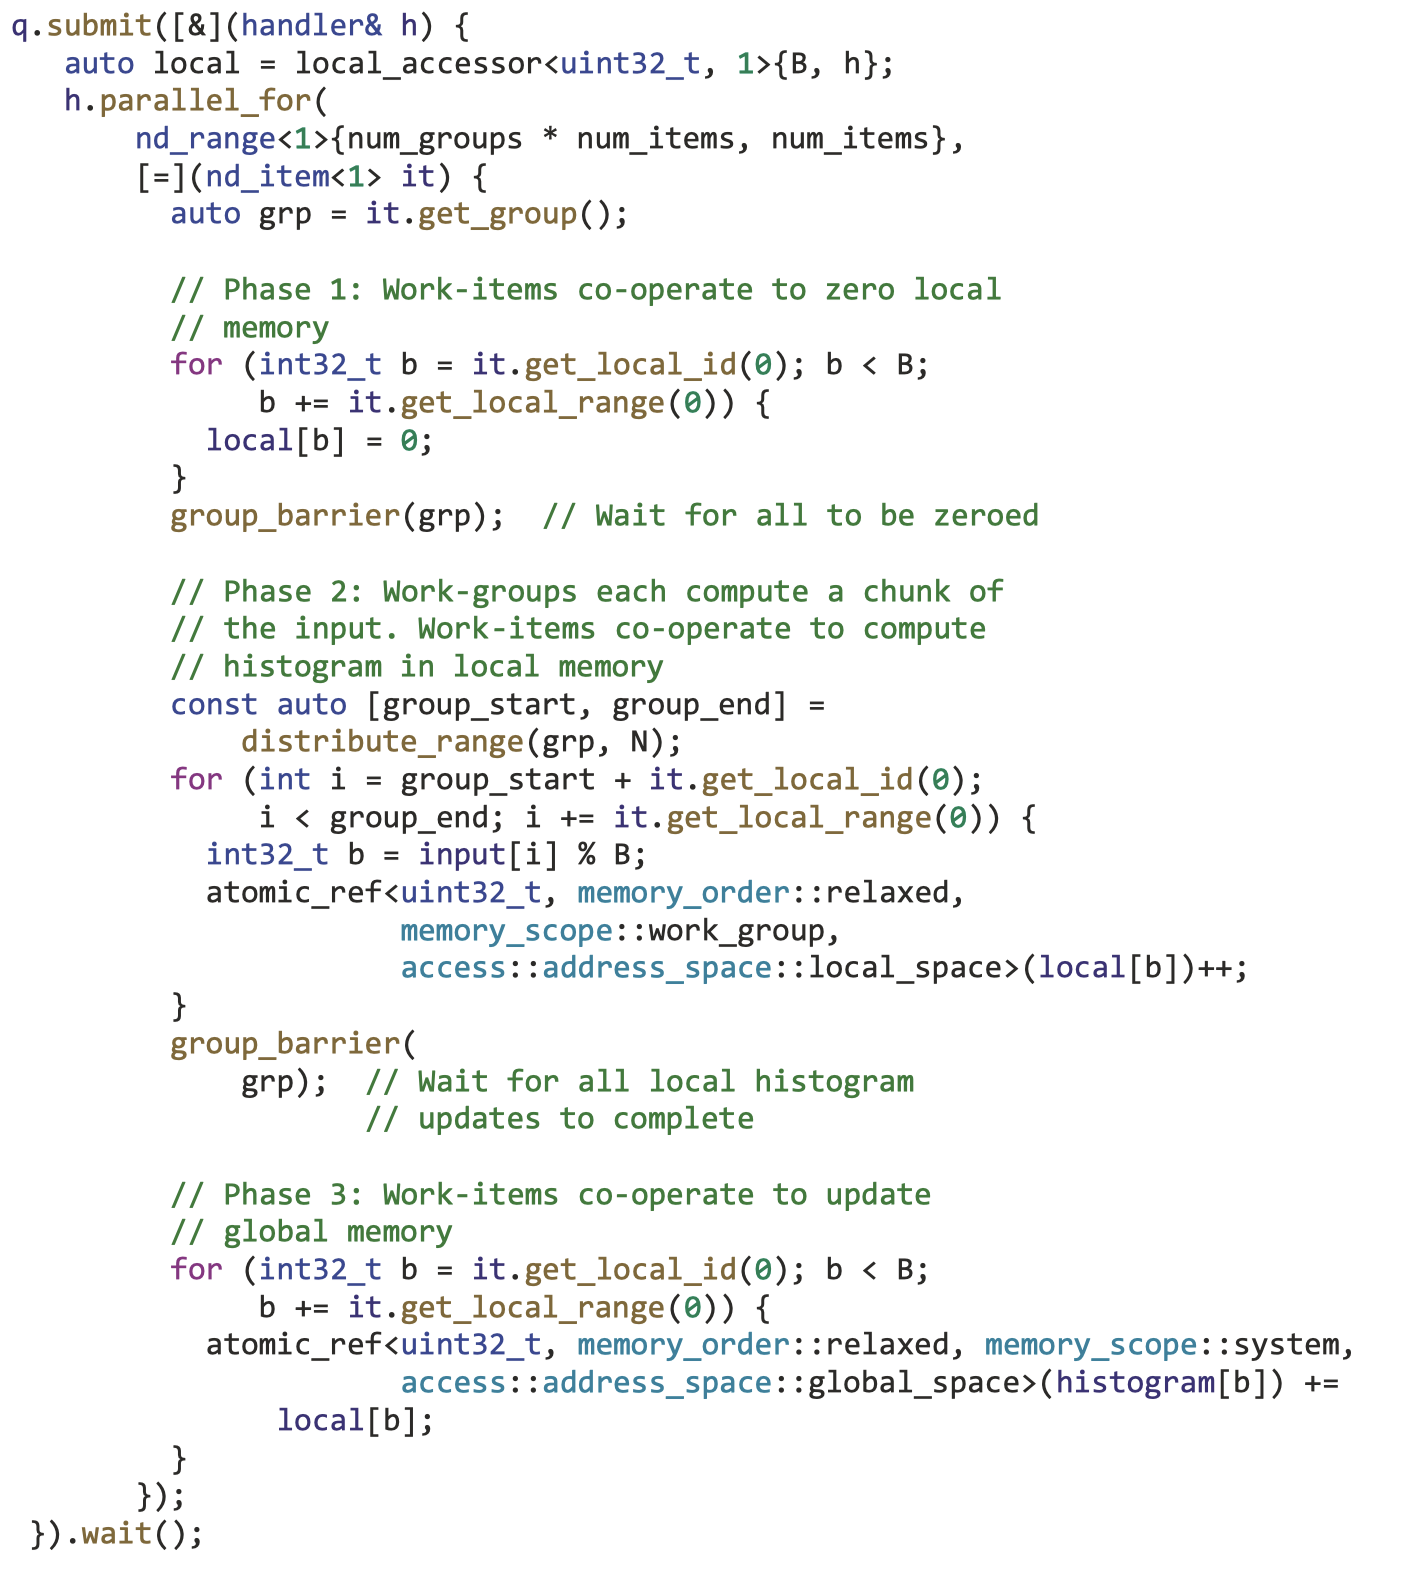
\includegraphics[width=0.9\textwidth]{figs/F19.17.png}
	\caption{\textit{使用不同内存空间中的原子引用计算直方图 }}
\end{figure}

图 19-17 中的代码演示了如何将宽松原子与Work-Groups Barrier结合使用来计算直方图。 
Kernel被Barrier分为三个阶段,每个阶段都有自己的原子性要求。 
请记住,Barrier既充当同步点又充当获取-释放栅栏,
这确保了一个阶段中的任何读取和写入对于后续阶段中Work-Groups中的所有Work-Items都是可见的。

第一阶段将某些Work-Groups本地内存的内容设置为零。 
每个Work-Groups中的Work-Items按照设计更新Work-Groups本地内存中的独立位置——不会发生竞争条件,并且不需要原子性。

第二阶段将部分直方图结果累积在本地存储器中。 
同一Work-Groups中的Work-Items可以更新Work-Groups本地内存中的相同位置,
但同步可以推迟到阶段结束——我们可以使用 memory\_order::relaxed 
和 memory\_scope::work\_group 来满足原子性要求 。

第三阶段将部分直方图结果贡献到存储在全局存储器中的总数中。 
同一Work-Groups中的Work-Items保证从Work-Groups本地内存中的独立位置读取,
但可能会更新全局内存中的相同位置——我们不再要求Work-Groups本地内存的原子性,
并且可以满足原子性 像以前一样使用 memory\_ order::relaxed 和 memory\_scope::system 对全局内存的要求。

\subsubsection{实现设备范围的同步}
回到第 4 章,我们警告不要编写试图跨Work-Groups同步Work-Items的Kernel。 
然而,我们完全预计本章的一些读者会渴望在原子操作之上实现他们自己的设备范围同步例程,并且我们的警告将被忽略。

\begin{remark}
	设备范围的同步目前是不可移植的,最好留给专业程序员。SYCL 的未来版本将解决这个问题。
\end{remark}

本节中讨论的代码很危险,不应期望在所有设备上都能工作,因为设备硬件功能和 SYCL 实现之间存在潜在差异。 
原子提供的内存排序保证与转发进度保证正交,并且在撰写本文时,SYCL 中的Work-Groups调度完全是实现定义的。 
正式化描述 SYCL ND 范围执行模型所需的概念和术语以及与Work-Items、
Sub-Groups和Work-Groups相关的前进进度保证是目前活跃的学术研究领域 - 
预计将构建 SYCL 的未来版本 在此工作上提供额外的调度查询和控制。 目前,这些主题应被视为仅供专家讨论。

\begin{figure}[H]
	\centering
	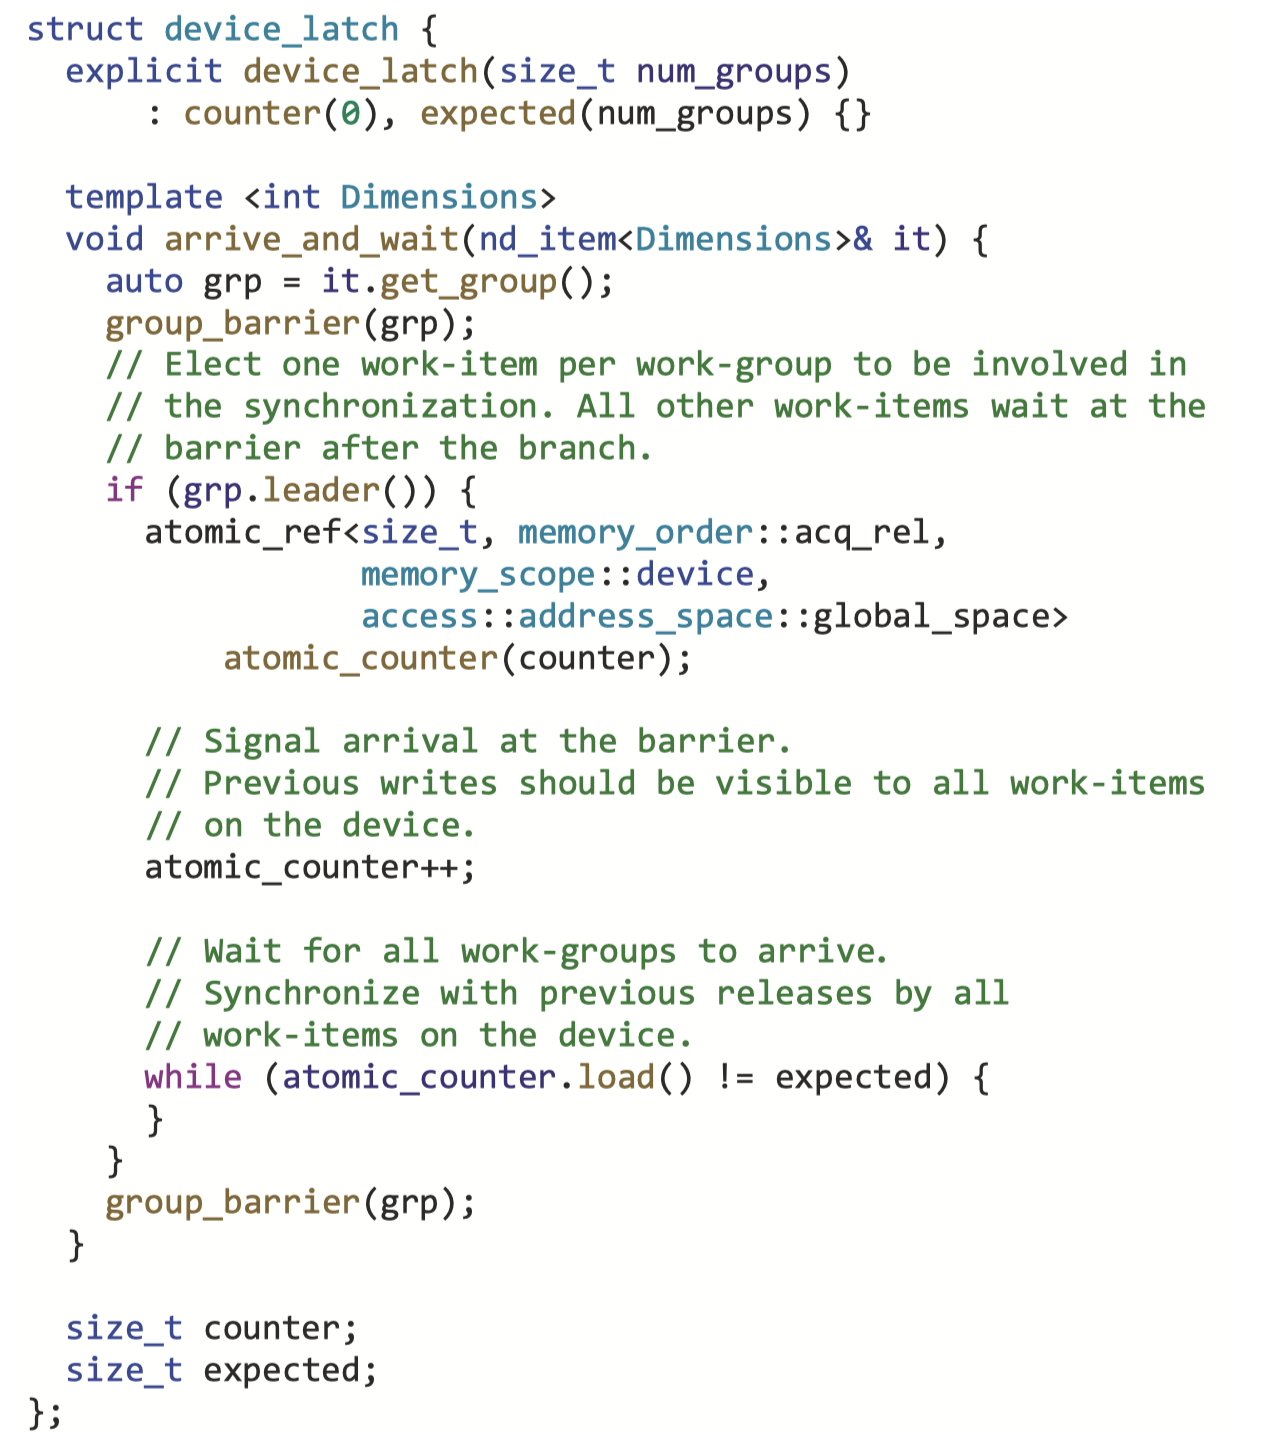
\includegraphics[width=0.9\textwidth]{figs/F19.18.png}
	\caption{\textit{在原子引用之上构建一个简单的器件范围锁存器 }}
\end{figure}

\begin{figure}[H]
	\centering
	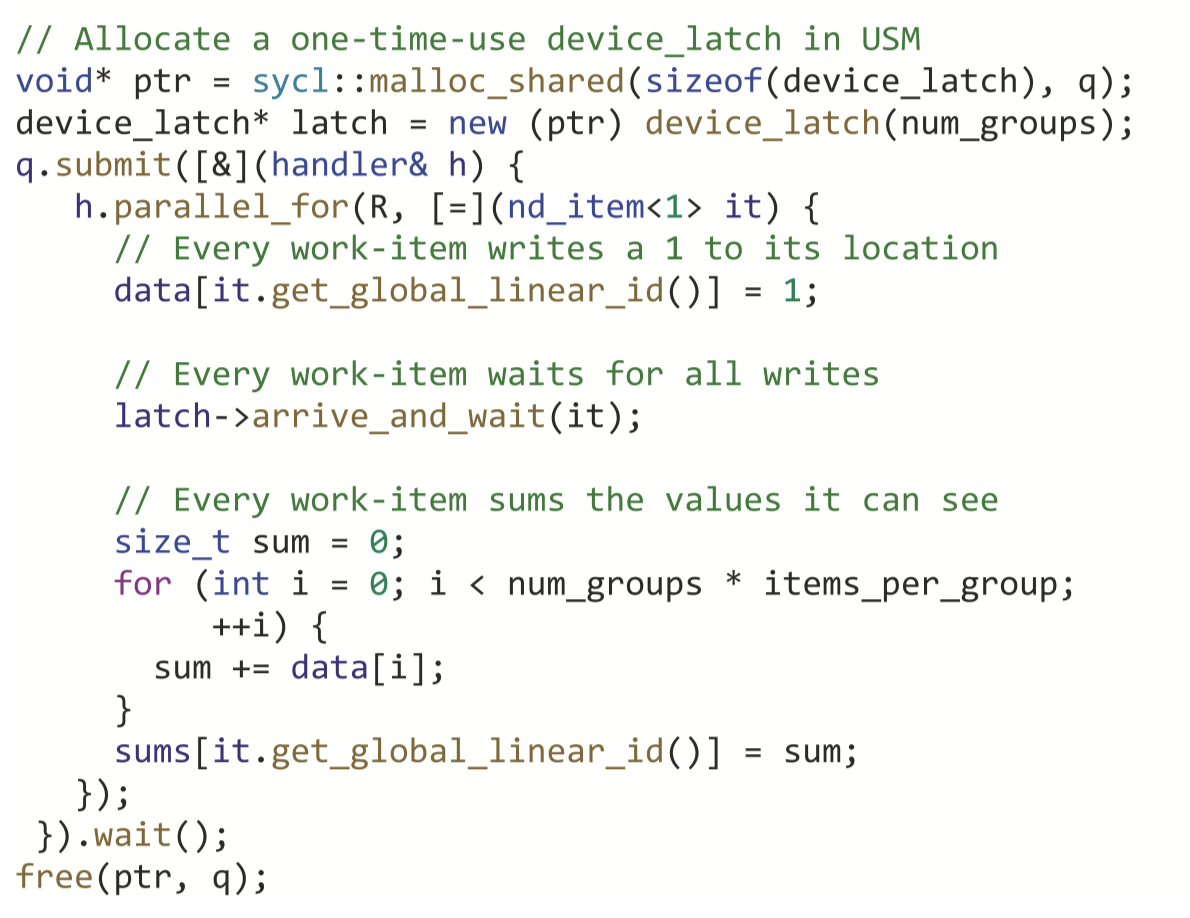
\includegraphics[width=0.9\textwidth]{figs/F19.19.png}
	\caption{\textit{使用图19-18中的器件范围锁存器 }}
\end{figure}

图 19-18 显示了设备范围锁存器(一次性Barrier)的简单实现,图 19-19 显示了其用法的简单示例。 
每个Work-Groups选择一个Work-Items来发出该组到达锁存器的信号,并使用朴素的自旋循环等待其他组的到达,
而其他Work-Items则使用Work-Groups Barrier等待选定的Work-Items 。 
正是这种自旋循环使得设备范围的同步不安全; 
如果任何Work-Groups尚未开始执行或当前正在执行的Work-Groups未公平调度,则代码可能会死锁。

\begin{remark}
	在没有足够强的前向进度保证的情况下,仅依靠内存顺序来实现同步原语可能会导致死锁!
\end{remark}

为了使代码正确运行,必须满足以下三个条件:

\begin{enumerate}
	\item 原子操作必须使用至少与所示一样严格的内存顺序,以保证生成正确的栅栏。

	\item NDrange 中每个Work-Groups的当选领导者必须独立于其他Work-Groups中的领导者取得进展,
	以避免单个Work-Items在循环中旋转,导致其他尚未增加计数器的Work-Items挨饿 。

	\item 设备必须能够同时执行ND范围内的所有Work-Groups,并具有强大的前进进度保证,
	以确保ND范围内每个Work-Groups的当选领导者最终到达闩锁。
\end{enumerate}

虽然此代码不保证可移植,但我们将其包含在这里是为了强调两个关键点:
(1)SYCL 具有足够的表达能力,可以实现特定于设备的调整,有时会牺牲可移植性; 
(2) SYCL 已经包含实现高级同步例程所需的构建块,这些例程可能会包含在该语言的未来版本中。

\subsection{概括}
本章对内存模型和原子类进行了高级介绍。 
了解如何使用(以及如何不使用!)这些类是开发正确、可移植且高效的并行程序的关键。

内存模型是一个极其复杂的主题,我们这里的重点是建立编写实际应用程序的基础。 
如果需要更多信息,可以参考下面引用的一些专门针对内存模型的网站、书籍和讲座。

\subsubsection{了解更多信息}
• A. Williams,《C++ 并发实践:实用多线程》,Manning,2012 年,978-1933988771

• H. Sutter,“原子<>武器:C++ 内存模型和现代硬件”,herbsutter.com/2013/02/11/atomic-weapons-the-c-memory-model-and-modernhardware/

• H-J。 Boehm,“Temporarily discourage memory\_order\_consume”,wg21.link/p0371

• C++ 参考,“std::atomic”,en.cppreference.com/w/cpp/atomic/atomic

• C++ 参考,“std::atomic\_ref”,en.cppreference.com/w/cpp/atomic/atomic\_ref